% Using XeTeX, produce a standalone pdf of the development process.
\documentclass{standalone}

\usepackage{tikz}
\usepackage{pgfplots}
\usetikzlibrary{shapes,fit,matrix,backgrounds,arrows,arrows.meta,positioning,chains,patterns,overlay-beamer-styles}
\tikzset{> = {Straight Barb[]}}
\pgfplotsset{compat = 1.14}

\usepackage{fontspec}
\setmainfont[ItalicFont={Fira Sans Light Italic},%
             BoldFont={Fira Sans},%
             BoldItalicFont={Fira Sans Italic}]%
            {Fira Sans Light}%

\definecolor{c1}{HTML}{006C71}
\definecolor{c2}{HTML}{005155}
\definecolor{c3}{HTML}{FF8928}
\definecolor{c4}{HTML}{E86900}

\begin{document}

  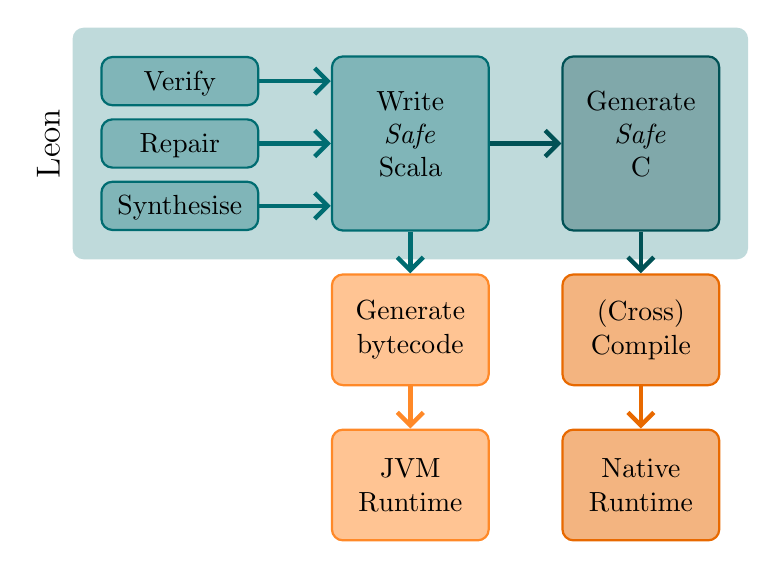
\begin{tikzpicture}
    [auto,
     commonbox/.style = {
       rectangle, draw = #1, thick, fill = #1!50,
       text width = 5em, text centered, rounded corners,
     },
     phantom1/.style = {
       text depth = .5ex, text height = 2ex,
     },
     phantom2/.style = {
       align = center, anchor = center,
       minimum height = 4em,
     },
     box1/.style = {
       commonbox = #1,
       phantom1,
     },
     box2/.style = {
       commonbox = #1,
       phantom2,
     },
    ]

    \matrix (m) [%
      column sep = 6ex, row sep = 1ex,
      matrix of nodes,
      nodes in empty cells,
      nodes = { },
    ] {%
      |[box1 = c1]| {Verify}     & |[phantom1]|                      & |[phantom1]|                     \\
      |[box1 = c1]| {Repair}     & |[phantom1]|                      & |[phantom1]|                     \\
      |[box1 = c1]| {Synthesise} & |[phantom1]|                      & |[phantom1]|                     \\
      && \\ % empty line for spacing
      |[phantom2]|               & |[box2 = c3]| {Generate bytecode} & |[box2 = c4]| {(Cross)\\ Compile} \\
      && \\ % empty line for spacing
      |[phantom2]|               & |[box2 = c3]| {JVM Runtime}       & |[box2 = c4]| {Native Runtime}    \\
    };

    \node [fit = (m-1-2)(m-3-2), commonbox = c1, inner ysep = 0em] (scala) {Write\\ \emph{Safe}\\ Scala};
    \node [fit = (m-1-3)(m-3-3), commonbox = c2, inner ysep = 0em] (genc)  {Generate\\ \emph{Safe}\\ C};

    \begin{scope}[every node/.style={font=\small\itshape}, ultra thick, ->]
      \begin{scope}[c1]
        \draw (m-1-1.east) to (m-1-1-|scala.west);
        \draw (m-2-1.east) to (m-2-1-|scala.west);
        \draw (m-3-1.east) to (m-3-1-|scala.west);
        \draw (scala.south) to (m-5-2.north);
      \end{scope}
      \draw [c3] (m-5-2.south) to (m-7-2.north);

      \begin{scope}
        \draw [c2] (scala.east) to (genc.west);
        \draw [c2] (genc.south) to (m-5-3.north);
        \draw [c4] (m-5-3.south) to (m-7-3.north);
      \end{scope}
    \end{scope}

    \begin{pgfonlayer}{background}
      \node[fill = c1!50, opacity = .5, inner sep = 10pt, rectangle, rounded corners,
            fit = (m-1-1) (genc)] (leon) {};
      \node[font=\large, anchor = center, rotate = 90, yshift = 2ex] at (leon.west) {Leon};
    \end{pgfonlayer}
  \end{tikzpicture}

\end{document}

